% TODO: images are on counted
% TODO: OLAP, CRM, ERP в скорочення
\section{ЗАДАЧА МАРКЕТИНГОВОЇ РОЗВІДКИ}
\subsection{Огляд проблем МІС}
\subsubsection{Основні поняття}
В ході аналізу проблемної області був складений глосарій:
\begin{longEnumerate}
\item Маркетинг --- це інститути та процеси, що створюють, доставляють та обмінюють пропозиції, що мають ціну для клієнтів, партнерів та суспільства в цілому\cite{kotler14}.
\item Маркетингова інформаційна система або МІС (англ. {\it marketing information system, MkIS}) --- це сукупність людей та систем, що виконують процедури збирання, сортування, аналізу та оцінки інформації для підтримки прийняття маркетингових рішень \cite{kotler14}. МІС може входити до складу більш загальної системи підтримки прийняття керівних рішень, EIS (англ. {\it executive information system})
\item Маркетингове дослідження --- це систематичний збір та аналіз даних та висновків щодо конкретної ринкової ситуації, з якою зіткнулася компанія \cite{kotler14}.
\item Маркетинговий канал --- це сукупність взаємопов’язаних організацій, що надають можливість використання та споживання різних товарів та послуг \cite{stern}.
% Маркетингова розвідка
\end{longEnumerate}
\subsubsection{Маркетингова розвідка як складова МІС}
% навіщо потрібна маркетингова розвідка в МІС
% хто займається, що на вході. 1 абзац.
 
Маркетингова інформаційна система складається з трьох частин \cite{kotler14}: внутрішній облік, маркетингові дослідження та розвідка. Основною частиною є маркетингові дослідження, а внутрішній облік та розвідка забезпечують дослідників точною, ретроспективною та щоденною інформацією про ринок та діяльність компанії. Збиранням внутрішньої ретроспективної інформації займаються системи внутрішнього обліку --- системи класів ERP та CRM. А збір щоденної, актуальної інформації з зовнішньої середи виконує маркетингова розвідка. За допомогою інтернету, засобів масової інформації, спеціалізованих агенств та звітності, комунікацій з клієнтами, в процесі розвідки збирається важлива інформація про стан ринку та ринкові тенденції. Наприклад, маркетингова розвідка може проінформувати дослідників, що згідно з новими статистичними звітами, змінився середній вік населення, а за допомогою інтернету визначити динаміку цін продуктів компаній-конкурентів.

\begin{stdfigure}
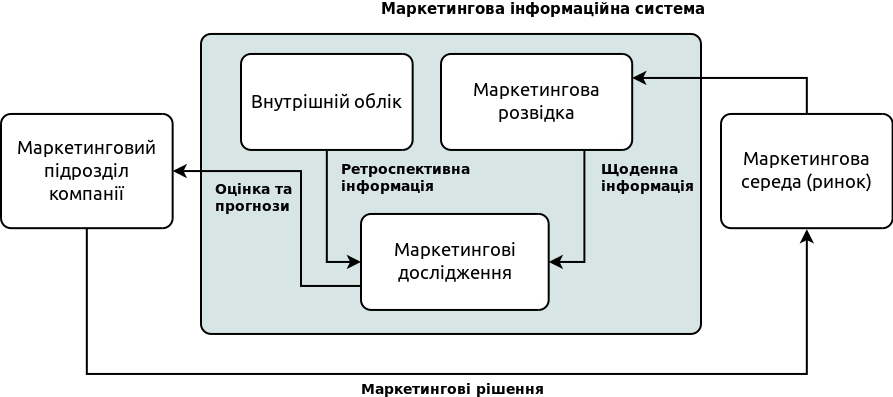
\includegraphics[width=7in]{images/mis_structure.png}
\caption{Структура МІС}
\label{fig:mis_structure}
\end{stdfigure}    

\subsubsection{Компоненти підсистеми маркетингової розвідки}
Формально, підстема маркетингової розвідки --- це процедури та джерела, які використовують маркетологи для збирання щоденної інформації про стан маркетингової середи\cite{kotler14}. Наразі, маркетингові інформаційні системи зосереджені на збиранні щоденної інформації та звітів про минулі періоди. Ця інформація допомагає дослідникам прогнозувати події на ринку та планувати власну маркетингову стратегію, але кінцева точність прогнозів сильно залежить від людського фактору, кваліфікації та досвіду аналітиків компанії.

Пропонується додати до підсистеми маркетингової розвідки складову (див. рис. \ref{fig:intelligence_scheme}), що буде автоматизувати процес прогнозування ринкової ситуації та надавати аналітикам перспективну інформацію. Автоматизація прогнозування дозволить скоротити витрати на маркетингові дослідження та збільшити точність прогнозів, що в свою чергу дозволить біль ефективно планувати діяльність компанії.

\begin{stdfigure}
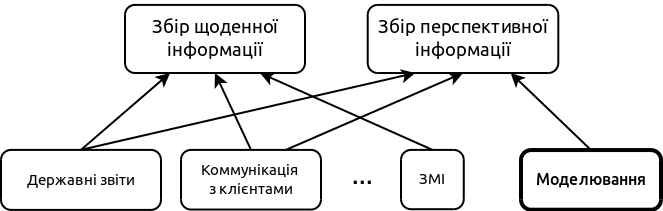
\includegraphics[width=7in]{images/intelligence_scheme.png}
\caption{Компоненти підсистеми маркетингової розвідки}
\label{fig:intelligence_scheme}
\end{stdfigure}    

\subsection{Бізнес-ігри}
\subsubsection{Поняття бізнес-гри}
% TODO: сорєц к "розповсюджені", в визначення [10], [6], класификація [36]
Моделювання економічних, бізнес-систем або бізнес-моделювання є розповсюдженою практикою, що використовується для навчання та аналізу. Розглянемо один з методів моделювання, бізнес-ігри. Бізнес-гра --- це процес послідовного або паралельного прийняття рішень учасниками ігри навколо деякої моделі бізнес-операції\cite{}; ігри складаються з ігроків, правил та ресурсів\cite{}. Ігри можуть бути класифікувані за: наявність конкуренції між учасниками, характером прийняття рішень (детермінований чи стохастичний), часовим інтервалом моделювання та ін.
% Что это такое: симуляция http://en.wikipedia.org/wiki/Business_simulation, состав игры, подразумевают, что участники будут принимать решения
\subsubsection{Моделювання маркетингових каналів}
% Маркетинговый канал может моделироваться играми типа: 1, 2, 3
% Маркетинговый канал -- это...
% Состоит из таких участников, связанных некоторым образом, потоки.
% преследование собственных интересов.
\subsubsection{Постановка задачі моделювання}

\subsection{Вимоги до ПЗ}
\subsubsection{Функціональні вимоги}
%TODO: use case, idef0

\subsubsection{Нефункціональні вимоги}
% 6 критеріїв ISO 
\subsection{Завдання на розробку ПЗ}